%%%%%%%%%%%%%%%%%%%%%%%%%%%%%%%%%%%%%%%%%%%%%%%%%%%%%%%%%%%
% --------------------------------------------------------
% Rho
% LaTeX Template
% Version 2.1.1 (01/09/2024)
%
% Authors: 
% Guillermo Jimenez (memo.notess1@gmail.com)
% Eduardo Gracidas (eduardo.gracidas29@gmail.com)
% 
% License:
% Creative Commons CC BY 4.0
% --------------------------------------------------------
%%%%%%%%%%%%%%%%%%%%%%%%%%%%%%%%%%%%%%%%%%%%%%%%%%%%%%%%%%%

\documentclass[9pt,a4paper,twoside]{rho-class/rho}
\usepackage[english]{babel}
\usepackage{amsmath}
% \usepackage{algorithmic} % Añade esto en el preámbulo
\usepackage{algorithm}
\usepackage{algpseudocode}
\usepackage{hyperref} % Para manejar URLs
\usepackage{biblatex} % Para el manejo de bibliografía

\addbibresource{rho.bib} 

%% Spanish babel recomendation
% \usepackage[spanish,es-nodecimaldot,es-noindentfirst]{babel}

\setbool{rho-abstract}{true} % Set false to hide the abstract
\setbool{corres-info}{false} % Set false to hide the corresponding author section

%----------------------------------------------------------
% TITLE
%----------------------------------------------------------

\journalname{Trabajo Final}
\title{ Quadtree }

%----------------------------------------------------------
% AUTHORS AND AFFILIATIONS
%----------------------------------------------------------

% \author[1]{Alberto Valentín Velásquez Santos}
% \author[2]{Rodolfo Morocho Caballero}
% \author[3]{Max Houston Ramirez Martel}
% \author[4]{Harold Mondragon Tavara}
\author[,$\dagger$]{Alberto Valentín Velásquez Santos}
\author[,$\dagger$]{Rodolfo Morocho Caballero}
\author[,$\dagger$]{Max Houston Ramirez Martel}
\author[,$\dagger$]{Harold Mondragon Tavara}

%----------------------------------------------------------

% \affil[1]{Alberto Valentín Velásquez Santos}
% \affil[2]{Rodolfo Morocho Caballero}
% \affil[3]{Max Houston Ramirez Martel}
% \affil[4]{Harold Mondragon Tavara}
\affil[$\dagger$]{Estos autores contribuyeron igualmente a este trabajo.}
%----------------------------------------------------------
% DATES
%----------------------------------------------------------

\dates{Este archivo fue compilado el 09 de Marzo del 2025}

%----------------------------------------------------------
% FOOTER INFORMATION
%----------------------------------------------------------

\leadauthor{Group The Bankers}
\footinfo{Creative Commons CC BY 4.0}
\smalltitle{\LaTeX\ Template}
\institution{Universidad de Tecnologia E Ingeniería}
\theday{March 09, 2025} %\today

%----------------------------------------------------------
% ARTICLE INFORMATION
%----------------------------------------------------------

% \corres{Provide the corresponding author information and publisher here.}
% \email{example@organization.com.}
% \doi{\url{https://www.doi.org/exampledoi/XXXXXXXXXX}}

\received{March 09, 2025}
\revised{March 09, 2025}
\accepted{March 09, 2025}
\published{March 09, 2025}
\license{Rho LaTeX Class \ccLogo\ This document is licensed under Creative Commons CC BY 4.0.}

%----------------------------------------------------------
% ABSTRACT
%----------------------------------------------------------

\begin{abstract}
    Este trabajo presenta un análisis detallado del algoritmo Quadtree, una estructura de datos jerárquica especializada en la subdivisión recursiva de espacios bidimensionales en cuadrantes. El Quadtree permite organizar y acceder eficientemente a datos espaciales, ofreciendo una complejidad logarítmica en operaciones como búsqueda, inserción y eliminación. A lo largo del documento, se exploran sus fundamentos teóricos, su implementación computacional y sus principales aplicaciones prácticas.
    La implementación de un Quadtree se basa en la representación de nodos que contienen información sobre coordenadas espaciales y referencias a nodos hijos correspondientes a los cuadrantes NW, NE, SW y SE. Se detallan algoritmos específicos para operaciones fundamentales como inserción y búsqueda, incluido el manejo de casos especiales como puntos ubicados en las líneas divisorias de los cuadrantes.
    Entre las aplicaciones destacadas se encuentra la detección de bordes en imágenes, donde el Quadtree facilita la segmentación mediante un proceso de tres fases: suavizado jerárquico, clasificación por clustering y refinamiento de bordes. Otra aplicación significativa es la detección de colisiones en entornos bidimensionales, donde el Quadtree reduce la complejidad computacional de $O(n^2)$ a $O(n \log n)$ al permitir verificar colisiones solo entre objetos ubicados en el mismo cuadrante o en cuadrantes adyacentes.
    Esta estructura de datos resulta particularmente valiosa en campos como gráficos por computadora, sistemas de información geográfica y procesamiento de imágenes, donde la eficiencia en el manejo de grandes volúmenes de datos espaciales es crucial.
\end{abstract}

%----------------------------------------------------------
\keywords{Quadtree, Estructura de datos jerárquica, Subdivisión espacial, Detección de bordes, Detección de colisiones, Complejidad computacional, Procesamiento de imágenes}
%----------------------------------------------------------

\begin{document}
	
%----------------------------------------------------------
% OPTIMIZATION PROBLEMS
%---------------------------------------------------------- 
    \maketitle
    \section{Introducción}

        \rhostart{L}os algoritmos de particionamiento espacial son fundamentales en el campo de la computación para organizar y manipular datos geométricos de manera eficiente. Entre estas estructuras destaca el Quadtree, una herramienta esencial que ha revolucionado el manejo de información espacial en múltiples dominios de aplicación.
        El Quadtree representa una aproximación jerárquica para la organización de datos bidimensionales, basada en el principio de "divide y vencerás". Esta estructura subdivide recursivamente un espacio en cuatro cuadrantes iguales, creando una representación en árbol donde cada nodo puede tener exactamente cuatro hijos. Esta característica permite que las operaciones de búsqueda, inserción y eliminación se realicen con una complejidad logarítmica respecto al número de elementos, superando significativamente a las estructuras de datos lineales tradicionales.
        En el presente trabajo exploraremos en profundidad el algoritmo Quadtree desde sus fundamentos teóricos hasta sus implementaciones prácticas. Analizaremos su estructura fundamental, los métodos de operación y las técnicas de optimización que lo hacen tan valioso. Especial atención merecen sus aplicaciones en áreas como el procesamiento de imágenes, donde facilita la detección de bordes y la segmentación, y en entornos interactivos como videojuegos, donde permite una detección de colisiones altamente eficiente.
        Los avances en hardware y la creciente demanda de aplicaciones que procesan grandes volúmenes de datos espaciales han renovado el interés por estas estructuras. Comprender las ventajas y limitaciones de los Quadtrees resulta esencial para ingenieros y científicos de datos que trabajan con representaciones espaciales y buscan optimizar el rendimiento de sus sistemas sin sacrificar la precisión en los resultados.

    \section{ Conceptos Fundamentales }
    El algoritmo Quadtree es una estructura de datos jerárquica que permite la subdivisión recursiva de un espacio bidimensional en cuadrantes más pequeños, este método permite organizar y acceder eficientemente a los datos, facilitando operaciones en aplicaciones como gráficos por computadora, sistemas de información geográfica y procesamiento de imágenes.
    \begin{figure}[h]
        \centering
        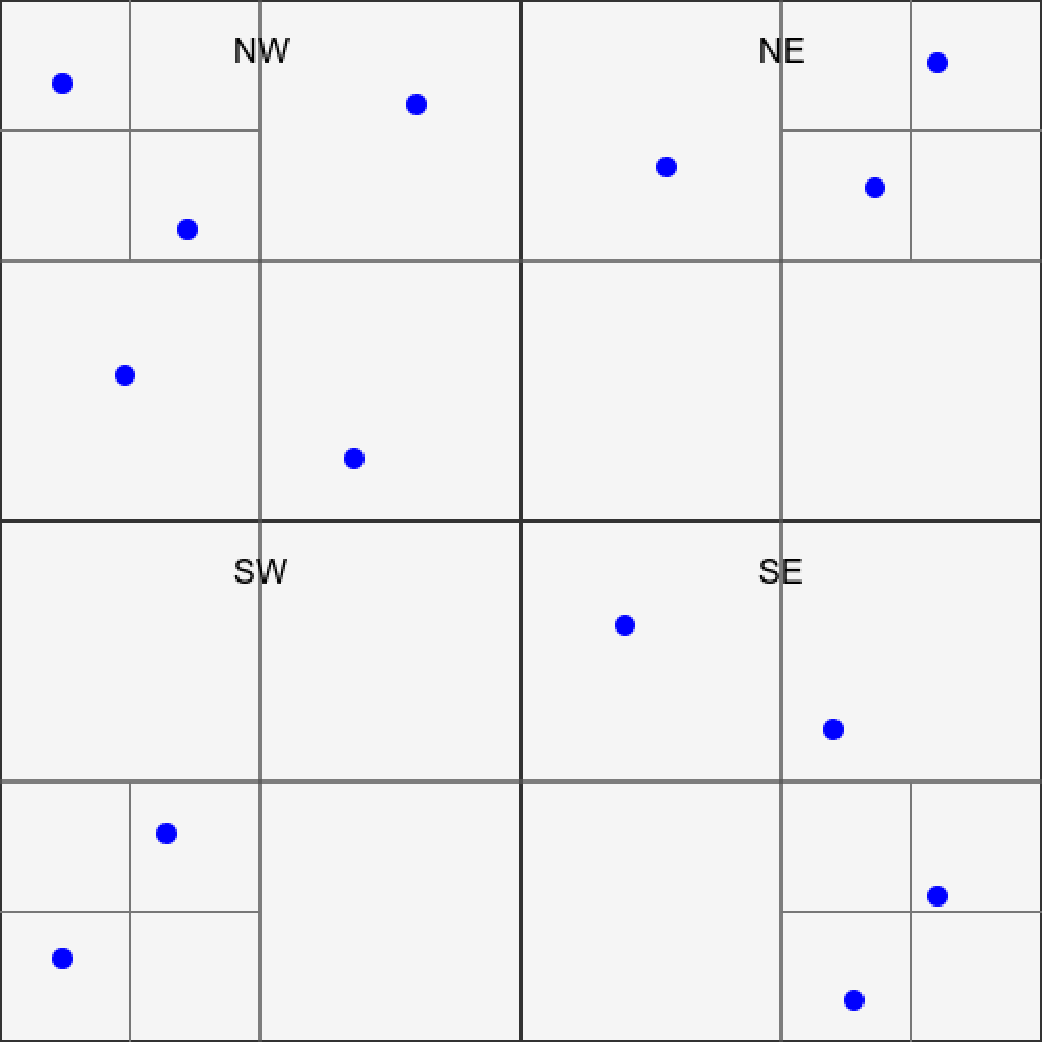
\includegraphics[width=\linewidth]{figures/quadtree.pdf}
        \caption{Representación grafica}
        \label{fig:representation_figure}
    \end{figure}\\
        \subsection{Fundamento}
            Quadtree tiene como principio fundamental la idea de \textit{divide y vencerás}, donde un problema complejo se descompone en subproblemas más fáciles de manipular y calcular, durante el proceso de división, este continúa hasta que se cumple una condición específica, como alcanzar una profundidad máxima o contener un número mínimo de elementos en una región.
            Matemáticamente, esta estructura permite una representación jerárquica del espacio, lo que facilita operaciones como búsqueda, inserción y eliminación de datos espaciales. La subdivisión recursiva en cuadrantes permite que las operaciones de búsqueda tengan una complejidad logarítmica en relación con el número de elementos, mejorando la eficiencia en comparación con estructuras de datos lineales, en otras palabras, se puede obtener mayor beneficio en términos de procesamiento, sin requerir tantas prestaciones en hardware y más rápido que otros algoritmos convencionales. (Hanan Samet)

        \subsection{Trabajos relacionados}
            El algoritmo es muy empleado en ciertas áreas de la computación como el procesamiento de imágenes, los Quadtrees facilitan la compresión y manipulación al dividir la imagen en regiones homogéneas, permitiendo una representación más compacta y eficiente. En el campo de visión computacional también tiene mucha utilidad, a modo de ejemplo se tiene el estudio de Miguel González que explica como los sensores de profundidad ofrecen nuevas oportunidades para aplicaciones de realidad aumentada o sistemas interactivos que requieran del cuerpo humano para realizar alguna acción, entonces en su investigación emplea Quadtrees para reducir el espacio de búsqueda de los algoritmos de agrupamiento, reduciendo las dimensiones elevadas de búsqueda y eliminar los espacios vacíos reduciendo la cantidad de búsquedas.

        \subsection{Segmentación basada en Quadtree}
            Otro ejemplo, es la segmentación basada en Quadtree para la detección de regiones homogéneas dentro de una imagen. Su enfoque se basa en tres componentes principales:
            \begin{itemize}
                \item Suavizado con Quadtree (Quad-tree smoothing)
                \item Clasificación (Classification)
                \item Estimación de bordes (Boundary estimation)
            \end{itemize}
            A través de estos tres pasos, el algoritmo busca reducir el ruido, clasificar los píxeles de la imagen de manera eficiente y refinar las fronteras entre regiones segmentadas.
            El primer componente, \textbf{Quad-tree smoothing}, aplica un proceso de suavizado jerárquico sobre la imagen. Cada nivel del Quadtree representa una versión más suavizada de la imagen, en la que cada nodo se obtiene promediando los valores de sus cuatro nodos hijos en el nivel anterior. Este procedimiento permite reducir la variabilidad de la calidad sin perder información estructural importante.
            En el segundo componente de \textbf{Clasificación}, la imagen en el nivel más alto del Quadtree se segmenta utilizando un algoritmo de clustering del centroide local. Este método no requiere información previa sobre el número de clases y agrupa los píxeles según sus estadísticas de nivel de gris, el algoritmo se ejecuta con diferentes tamaños de ventana, aceptando el resultado cuando las segmentaciones obtenidas son consistentes.
            El tercer componente, \textbf{Boundary estimation}, se encarga de refinar los bordes de las regiones segmentadas mediante un proceso descendente dentro de la jerarquía del Quadtree. Para ello, se define una región de borde donde la clasificación no es completamente segura. Los nodos fuera de esta región mantienen la clasificación del nivel superior, mientras que los nodos dentro del área se refinan utilizando un filtro de suavizado y un criterio de distancia mínima, reduciendo el ancho de los bordes progresivamente, hasta obtener la mayor resolución de la imagen. (M. Spann y R. Wilson)
%----------------------------------------------------------
%----------------------------------------------------------
% REAL CASES
%----------------------------------------------------------
    \section{Visualización y Representación}
        El quadtree se implementa como una generalización multidimensional de un árbol binario de búsqueda. En dos dimensiones, cada punto de datos se representa como un nodo en un quadtree en forma de un registro de tipo \textbf{nodo} que contiene siete campos. Los primeros cuatro campos contienen punteros a los cuatro hijos del nodo correspondientes a las direcciones (es decir, cuadrantes) NW, NE, SW y SE. Si $P$ es un puntero a un nodo y $i$ es un cuadrante, entonces estos campos se referencian como $\text{SON}(P, i)$. Podemos determinar el cuadrante específico en el que se encuentra un nodo, digamos $p$, en relación con su padre mediante el uso de la función $\text{SONTYPE}(P)$, que tiene un valor de $i$ si $\text{SON}(\text{FATHER}(P),i) = P$.
        $\text{XCOORD}$ e $\text{YCOORD}$ contienen los valores de las coordenadas $x$ e $y$, respectivamente, del punto de datos. El campo $\text{NAME}$ contiene información descriptiva sobre el nodo (por ejemplo, el nombre de la ciudad). Suponemos que cada punto de datos es único. Si una aplicación permite colisiones (es decir, varios puntos de datos con las mismas coordenadas), entonces la estructura de datos podría contener un campo adicional en el que se almacenaría un puntero a una lista de colisiones de desbordamiento. Se podría argumentar que dedicar un campo adicional a un evento poco frecuente, como una colisión, desperdicia almacenamiento; sin embargo, sin él, requeriríamos un procedimiento de inserción de nodos considerablemente más complicado.

        \subsection{Inserción}
            Los registros se insertan en árboles cuaternarios de puntos de una manera similar a la que se hace para los árboles de búsqueda binaria. En esencia, buscamos el registro deseado en función de sus coordenadas \(x\) e \(y\). En cada nodo se realiza una comparación mediante el uso del procedimiento \texttt{PT\_COMPARE} y se elige el subárbol apropiado para la siguiente prueba. Al llegar al final del árbol (es decir, cuando se encuentra un puntero \texttt{NIL}), encontramos la ubicación donde se insertará el registro. La inserción real se logra mediante el uso del procedimiento \texttt{PT\_INSERT}.
        
            Para manejar los puntos de datos que se encuentran directamente en una de las líneas del cuadrante que emanan de un punto de datos, digamos \(P\), adoptamos las mismas convenciones utilizadas para el método de cuadrícula; los límites inferior e izquierdo de cada bloque están cerrados, mientras que los límites superior y derecho de cada bloque están abiertos.
        \subsection{Búsqueda}
        \subsection{Búsqueda por Rango}
    %----------------------------------------------------------
%----------------------------------------------------------
% CONCLUTIONS
%----------------------------------------------------------        
    \section{Aplicaciones Prácticas}
        \subsection{Detección de Bordes usando Quad Tree}

        Un Quad Tree es una estructura de datos que divide un espacio 2D en cuatro cuadrantes iguales. Cada cuadrante puede subdividirse recursivamente, lo que permite una representación jerárquica de los datos espaciales. Esta estructura es especialmente útil para aplicaciones como la detección de bordes, ya que permite manejar grandes volúmenes de datos de manera eficiente al reducir la complejidad computacional.
        
            \subsubsection{Detección de Bordes}
            
            La detección de bordes es un proceso crítico en el análisis de imágenes, ya que permite identificar las transiciones entre diferentes regiones de una imagen. Un método comúnmente utilizado para la detección de bordes es el algoritmo de Canny, que se puede integrar con Quad Trees para mejorar la eficiencia y precisión en la segmentación.
            
            \subsubsection{Pasos para Implementar Detección de Bordes con Quad Trees}
            
            \begin{enumerate}
                \item \textbf{División Inicial:} Comienza dividiendo la imagen en cuadrantes utilizando el QuadTree. Esta división permite enfocarse en áreas más pequeñas y manejables.
                
                \item \textbf{Aplicación del Algoritmo de Detección de Bordes:} Para cada cuadrante, aplica el algoritmo de Canny o cualquier otro método adecuado para detectar bordes. Esto implica suavizar la imagen con un filtro Gaussiano y luego aplicar técnicas para encontrar los contornos.
                
                \item \textbf{Segmentación:} Una vez que se han detectado los bordes, se pueden segmentar los cuadrantes que contienen información relevante sobre los objetos en la imagen. Los cuadrantes vacíos o irrelevantes pueden ser descartados, optimizando así el proceso.
                
                \item \textbf{Manejo de Transiciones:} Es fundamental manejar adecuadamente las transiciones en los bordes, ya que esto puede afectar la calidad del análisis. Se deben establecer reglas para asegurar que los elementos generados sean válidos y representen correctamente el borde del objeto.
                
                \item \textbf{Revisión y Refinamiento:} Finalmente, revisa los cuadrantes resultantes y refina la segmentación según sea necesario. Esto puede incluir la eliminación de elementos inválidos o la mejora de los ángulos y formas detectadas.
            \end{enumerate}
            
            \subsubsection{Ventajas del Uso de Quad Trees en Detección de Bordes}
            
            \begin{itemize}
                \item \textbf{Eficiencia Computacional:} Al dividir el espacio en cuadrantes, se reduce la cantidad de datos a procesar en cada paso.
                
                \item \textbf{Escalabilidad:} La estructura permite manejar imágenes grandes sin comprometer el rendimiento.
                
                \item \textbf{Flexibilidad:} Se puede adaptar a diferentes tipos de imágenes y requisitos específicos del análisis.
            \end{itemize}
            
            En resumen, la detección de bordes utilizando Quad Trees combina la eficiencia estructural con técnicas avanzadas de procesamiento de imágenes, lo que resulta en un método poderoso para segmentar y analizar objetos dentro de imágenes digitales.
            \begin{figure}[h]
                \centering
                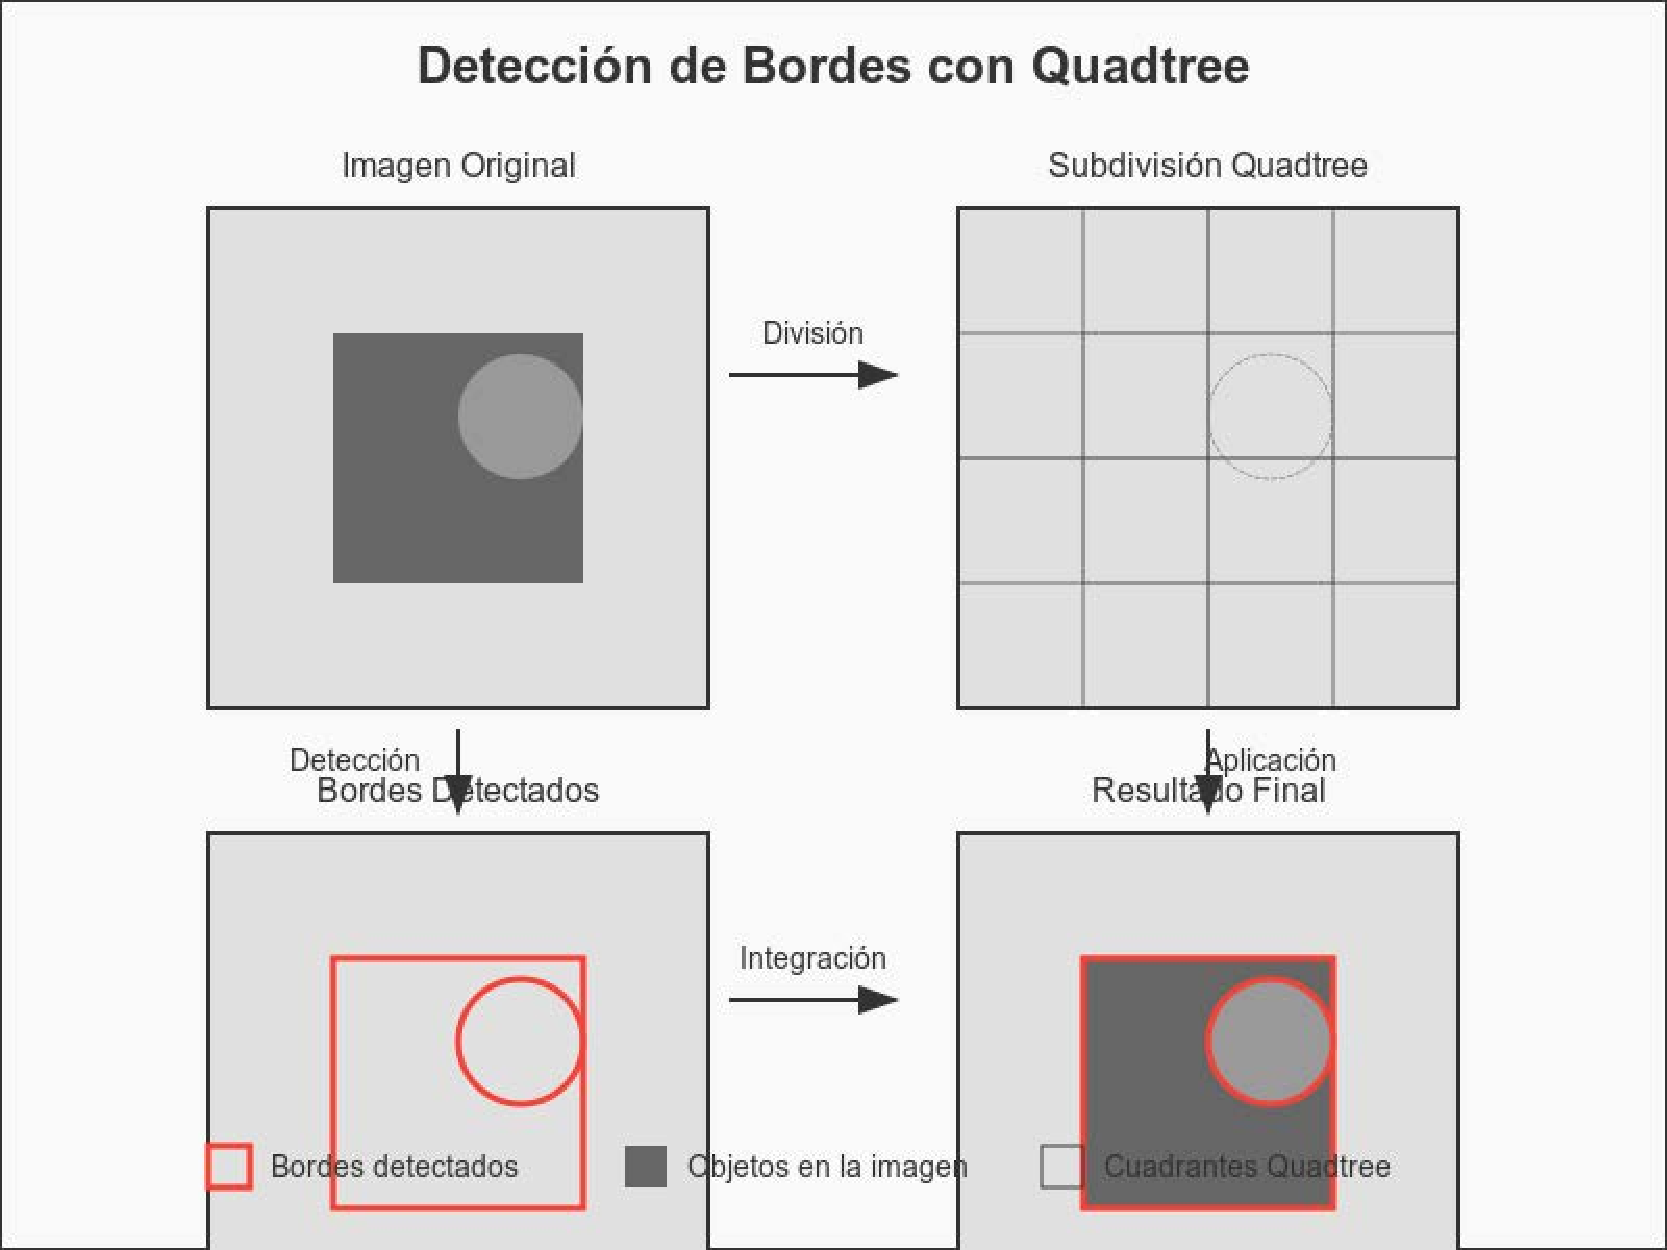
\includegraphics[width=\linewidth]{figures/edge-detection.pdf}
                \caption{Representación grafica de detección de bordes} 
                \label{fig:deteccion_figure}
            \end{figure}
        \subsection{Detección de colisiones}

        La detección de colisiones usando Quad Trees es una técnica eficiente para manejar la interacción entre múltiples objetos en un entorno 2D, especialmente en aplicaciones como videojuegos.

        Un Quadtree es una estructura de datos jerárquica que divide un espacio bidimensional en cuatro cuadrantes o nodos hijos. Cada nodo puede contener objetos y, si el número de objetos en un cuadrante excede un límite predefinido, ese cuadrante se subdivide nuevamente en cuatro partes. Este enfoque permite gestionar grandes cantidades de objetos sin necesidad de verificar cada posible colisión entre ellos, lo que sería computacionalmente costoso.

        \subsubsection{Funcionamiento}
        \begin{itemize}
            \item \textbf{División del espacio:} El espacio se divide inicialmente en cuatro cuadrantes. Cada cuadrante puede contener múltiples objetos.
            
            \item \textbf{Subdivisión:} Si un cuadrante contiene más de un número determinado de objetos (por ejemplo, 10), se subdivide en cuatro nuevos cuadrantes. Este proceso puede repetirse hasta alcanzar una profundidad máxima deseada.
            
            \item \textbf{Comprobación de colisiones:} Al realizar la detección de colisiones, cada objeto solo necesita verificar colisiones con otros objetos dentro de su mismo cuadrante o los cuadrantes adyacentes, reduciendo significativamente el número de verificaciones necesarias.
        \end{itemize}

        \subsubsection{Ventajas del uso de Quad Trees}
        \begin{itemize}
            \item \textbf{Reducción del costo computacional:} En lugar de realizar $O(n^2)$ comprobaciones (donde $n$ es el número de objetos), el uso de Quad Trees puede reducir este número a $O(n\log n)$ o incluso menos, dependiendo de la distribución espacial de los objetos.
            
            \item \textbf{Eficiencia en escenarios dinámicos:} En entornos donde los objetos se mueven constantemente, los Quad Trees pueden actualizarse rápidamente al mover objetos entre cuadrantes según sea necesario.
            
            \item \textbf{Facilidad para manejar diferentes escalas:} Los Quad Trees son útiles para manejar diferentes tamaños y formas de objetos, permitiendo que las comprobaciones sean más precisas.
        \end{itemize}

        \subsubsection{Implementación práctica}
        Para implementar un Quadtree para la detección de colisiones:

        \begin{itemize}
            \item \textbf{Definir la estructura del nodo:} Cada nodo debe contener información sobre su área (rectángulo delimitador), una lista de objetos y referencias a sus nodos hijos.
            
            \item \textbf{Método para insertar objetos:} Implementar un método que coloque un objeto en el nodo correspondiente y que subdivida el nodo si es necesario.
            
            \item \textbf{Método para comprobar colisiones:} Crear una función que verifique las colisiones solo con los objetos dentro del mismo nodo o nodos adyacentes.
            
            \item \textbf{Actualizar posiciones:} Al mover objetos, se debe actualizar su posición en el Quadtree para asegurar que siempre estén en el nodo correcto.
        \end{itemize}
        \begin{figure}[h]
            \centering
            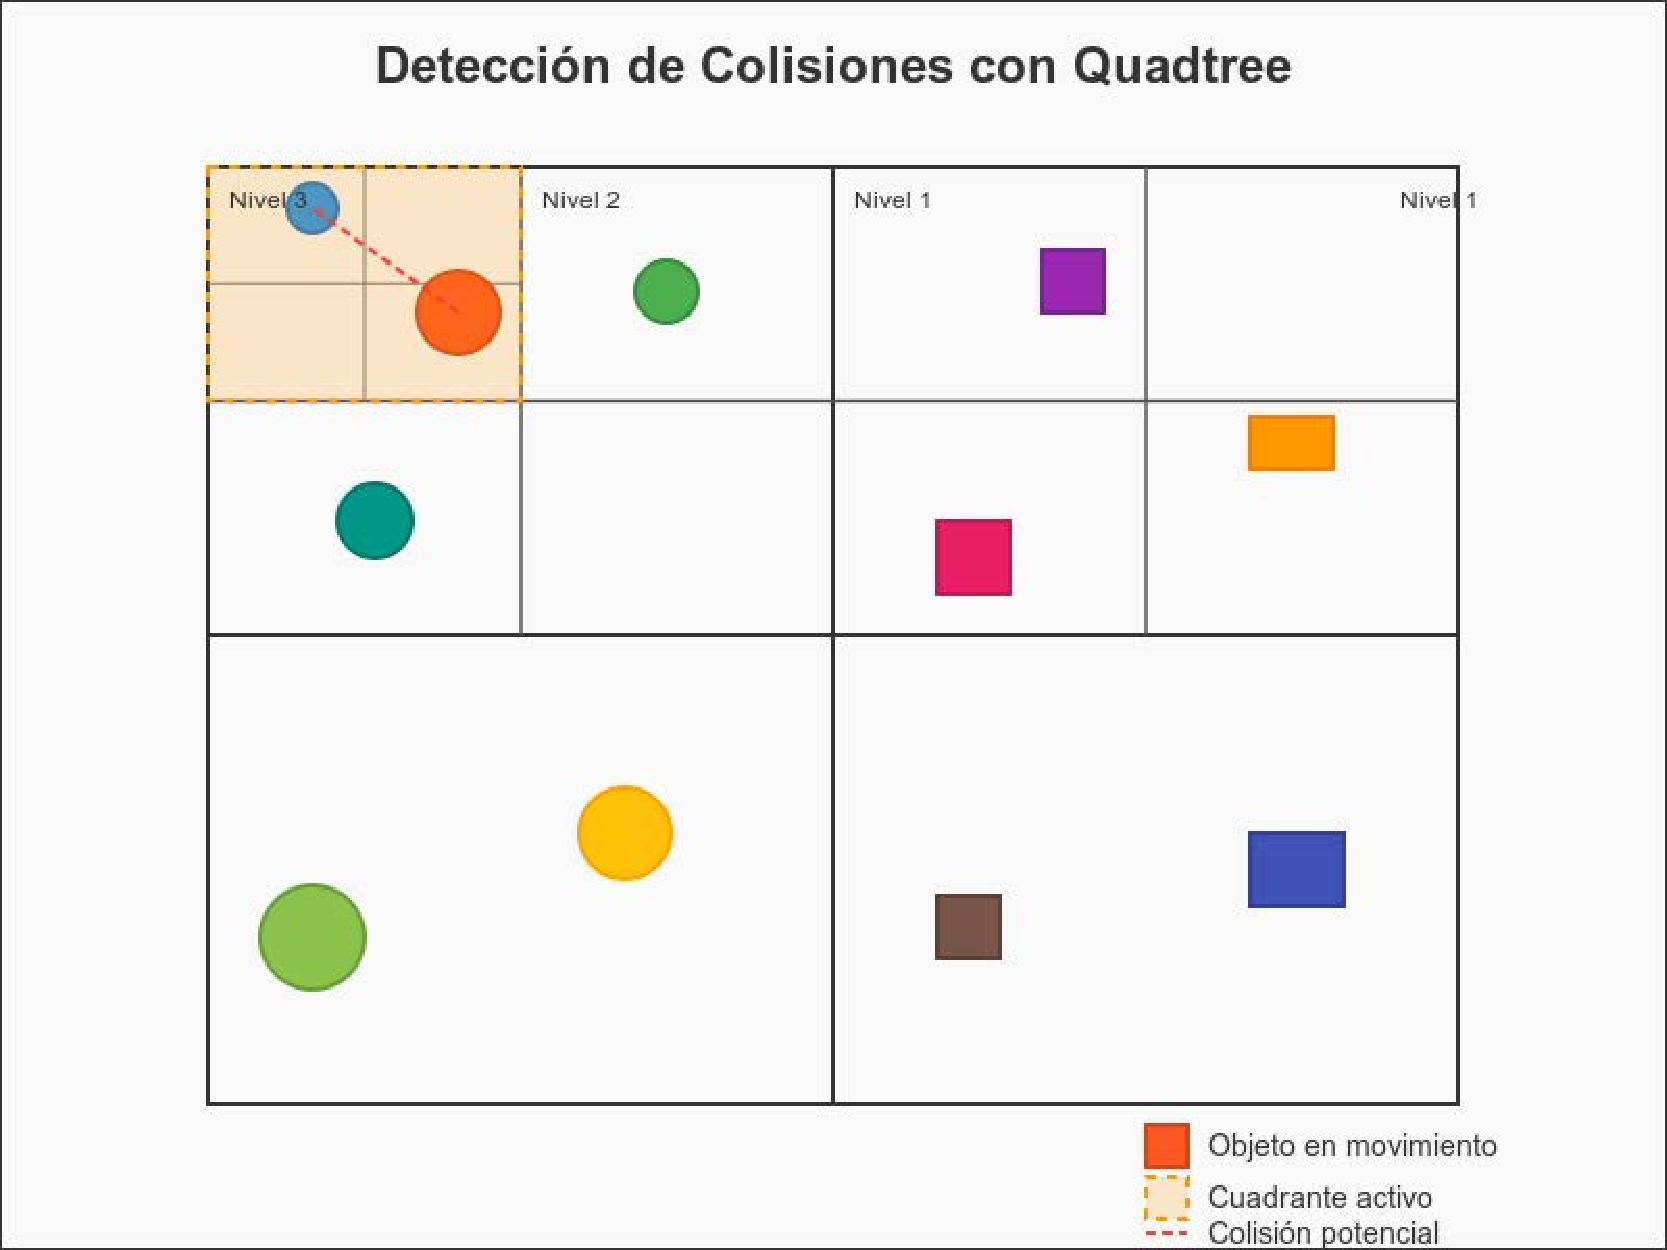
\includegraphics[width=\linewidth]{figures/quadtree-collision.pdf}
            \caption{Representación grafica de colisiones} 
            \label{fig:colision_figure}
        \end{figure}
        \section{Limitaciones}
        
    \section{Conclusiones}

        \begin{itemize}
        \item Es uno de las mejores estructuras de datos para almacenar grandes volumenes de información
        \end{itemize}
    
    \defbibheading{bibliography}{\section*{Referencias}}
    \printbibliography
 
%----------------------------------------------------------
% CONTENTS
%----------------------------------------------------------
    \renewcommand{\contentsname}{Tabla de Contenidos}
    \tableofcontents
    \linenumbers
%----------------------------------------------------------

    % \printbibliography

%----------------------------------------------------------    

\end{document}